\documentclass[11pt]{article}
% Shared preamble for the expert and beginner reports.
\usepackage[T1]{fontenc}
\usepackage[utf8]{inputenc}
\usepackage{lmodern}
\usepackage{microtype}
\DisableLigatures{encoding = T1, family = tt*}  % keep -- as two hyphens in code
\usepackage[a4paper,margin=2.3cm]{geometry}
\usepackage{amsmath,amssymb}
\usepackage{graphicx}
\usepackage{booktabs,longtable,multirow,makecell}
\usepackage{float}
\usepackage{caption}
\usepackage{subcaption}
\usepackage{enumitem}
\usepackage{xcolor}
\usepackage{tikz}
\usetikzlibrary{arrows.meta,positioning,shapes.geometric,calc,decorations.pathreplacing}
\usepackage{algorithm}
\usepackage{algpseudocode}
\usepackage{listings}
\usepackage[most]{tcolorbox}
\usepackage{fancyhdr}
\usepackage[hidelinks]{hyperref}

\graphicspath{{../figures/}}
\setlength{\parskip}{0.45em}
\setlength{\parindent}{0pt}
\setlength{\emergencystretch}{3em}  % long code identifiers: loosen lines instead of overflowing
\setlist{itemsep=0.15em,topsep=0.3em}
\renewcommand{\arraystretch}{1.15}

\definecolor{codebg}{RGB}{246,246,248}
\definecolor{codekw}{RGB}{0,72,150}
\definecolor{codecm}{RGB}{110,110,110}
\definecolor{codestr}{RGB}{140,40,20}
\definecolor{warn}{RGB}{176,64,0}
\definecolor{okc}{RGB}{0,110,60}
\definecolor{boxblue}{RGB}{225,236,250}
\definecolor{boxamber}{RGB}{253,240,215}
\definecolor{boxgreen}{RGB}{226,244,230}
\definecolor{boxgray}{RGB}{238,238,238}

\lstdefinestyle{py}{language=Python,basicstyle=\ttfamily\footnotesize,keywordstyle=\color{codekw}\bfseries,
  commentstyle=\color{codecm}\itshape,stringstyle=\color{codestr},backgroundcolor=\color{codebg},
  frame=single,rulecolor=\color{gray!40},breaklines=true,breakatwhitespace=false,columns=fullflexible,
  keepspaces=true,showstringspaces=false,xleftmargin=0.5em,xrightmargin=0.5em,aboveskip=0.6em,belowskip=0.6em}
\lstdefinestyle{sh}{basicstyle=\ttfamily\footnotesize,backgroundcolor=\color{codebg},frame=single,
  rulecolor=\color{gray!40},breaklines=true,columns=fullflexible,keepspaces=true,showstringspaces=false,
  xleftmargin=0.5em,xrightmargin=0.5em,aboveskip=0.6em,belowskip=0.6em}
\lstset{style=py}

\newtcolorbox{keybox}[1][]{colback=boxblue,colframe=codekw!70,boxrule=0.5pt,arc=2pt,left=6pt,right=6pt,top=4pt,bottom=4pt,fonttitle=\bfseries,#1}
\newtcolorbox{warnbox}[1][]{colback=boxamber,colframe=warn,boxrule=0.5pt,arc=2pt,left=6pt,right=6pt,top=4pt,bottom=4pt,fonttitle=\bfseries,#1}
\newtcolorbox{okbox}[1][]{colback=boxgreen,colframe=okc,boxrule=0.5pt,arc=2pt,left=6pt,right=6pt,top=4pt,bottom=4pt,fonttitle=\bfseries,#1}
\newtcolorbox{notebox}[1][]{colback=boxgray,colframe=gray!60,boxrule=0.5pt,arc=2pt,left=6pt,right=6pt,top=4pt,bottom=4pt,fonttitle=\bfseries,#1}

% Notation
\newcommand{\kT}{k_{\mathrm{B}}T}
\newcommand{\xiP}{\xi_{P}}
\newcommand{\gl}{\gamma_{l}}
\newcommand{\Pe}{\mathrm{Pe}}
\newcommand{\Flex}{\mathfrak{F}}
\newcommand{\spn}{\mathfrak{s}}
\newcommand{\dd}{\mathrm{d}}
\newcommand{\vect}[1]{\mathbf{#1}}
\newcommand{\code}[1]{\texttt{\detokenize{#1}}}
\newcommand{\NR}{\textbf{not a replication}}

\pagestyle{fancy}
\fancyhf{}
\renewcommand{\headrulewidth}{0.3pt}
\fancyfoot[C]{\thepage}

\fancyhead[L]{\small Self-propelled worm-like filaments: controlled reproduction}
\fancyhead[R]{\small Expert report}

\title{\textbf{Controlled Reproduction of Isele-Holder, Elgeti \& Gompper (2015)}\\[0.3em]
\large Self-propelled worm-like filaments: model, integrator audit, observables,\\ formation gate, and the first $5\tau$ trajectory\\[0.5em]
\normalsize Expert report (technical record of all work to date)}
\author{Prepared with Claude Code for the spin-chain-polymer project}
\date{5 October 2026}

\begin{document}
\maketitle
\thispagestyle{empty}

\begin{abstract}
\noindent
We document a controlled reproduction effort of R.~E.~Isele-Holder, J.~Elgeti and G.~Gompper,
\emph{Soft Matter} \textbf{11}, 7181 (2015), DOI 10.1039/c5sm01683e: a two-dimensional, overdamped,
bead--spring worm-like chain propelled homogeneously along its tangent. Starting from an audited
Python/Numba tree (``v2''), we (i) verified the force law against the published PDF and the arXiv
\LaTeX{} source, (ii) found and removed a silent centre-of-mass recentering that corrupted every stored
frame for the dynamics observables, (iii) established the index convention that maps the paper's
leading bead onto the code, (iv) implemented and unit-tested the inputs of Figures~2--10
(spiral number, symmetrized kurtosis, railway MSD, mean-square rotation, centre-of-mass MSD,
dynamic structure factor), (v) built segment-safe checkpoint/resume, stitching and a verdict program,
(vi) ran a formation gate that showed spiral formation over 10 contour lengths is decided by the noise
realisation (seed), not by the non-bonded exclusion policy, and (vii) completed one $5\tau$ trajectory
at the strong-spiral point ($\Pe=5000$, $\xiP/L=0.2$, $N=100$, seed 12013, \code{paper_all_pairs}).
On the window $0.5$--$5\tau$ the spiral number satisfies $|\spn|>2$ for $97.8\%$ of samples,
the symmetrized kurtosis is $\beta_2=1.03$, and the longest uninterrupted plateau lasts at least
$2007.75$ contours (censored by the end of the run). The pre-registered description is
\emph{predominant on this seed only}. This is \NR: one seed, one Figure-2 point, an unpublished
timestep, and an unresolved exclusion policy.
\end{abstract}

\begin{keybox}[title=Status in one table]
\begin{tabular}{@{}p{0.04\linewidth}p{0.36\linewidth}p{0.52\linewidth}@{}}
\toprule
& Stage & State \\ \midrule
1 & Force law & Done. Verified against PDF and arXiv source. \\
2 & Observables (schema 3) & Done. 64 unit tests pass. \\
3 & Formation (10 contours) & Partial: seed 12013 winds under both policies, seed 12003 under neither. \\
4 & Fig.~2c: $>5\tau$, spiral predominant & One trajectory complete: predominant, seed 12013 only. \\
5 & Fig.~2a--b and Figs.~6, 8--10 at paper length & Not started (primitives exist). \\
6 & Phase diagram (Fig.~4e) & Blocked: ESI timestep and \code{special_bonds} line unavailable. \\ \bottomrule
\end{tabular}
\end{keybox}

\tableofcontents
\newpage

%=====================================================================
\section{Scope, provenance and conventions}
%=====================================================================
\subsection{Objective and rules of engagement}
The task was a \emph{controlled reproduction}: make an existing simulator able to generate the
observables of the paper's Figures~2--10 \emph{without changing the force law}, then produce
paper-duration trajectories from which a second program (not the simulator) computes those curves.
The following rules held throughout and are binding on everything reported here:
\begin{itemize}
\item No retuning of $\kappa$, $f_p$, $\Delta t$ or the noise; no normalisation of the propulsion; no change of the
bending prefactor $1/4$; no flip of the force kernel.
\item No regime classifier based on excess kurtosis, end-to-end distance or a hand-set $|\spn|$ cut.
Descriptions are produced by fixed, pre-stated rules and reported as text, never as a pass bit
(Section~\ref{sec:verdict}).
\item Anything shorter than $5\tau$ after the transient is labelled \emph{not a replication}.
\item Numbers that exist only in the Electronic Supplementary Information (ESI)---the per-run timestep and
the LAMMPS input---are left as named placeholders, never invented.
\end{itemize}

\subsection{Sources}
\begin{itemize}
\item \code{c5sm01683e.pdf}: the published article (main text; Eqs.~1--29; Figs.~2,3,4,6,8,9,10).
\item \code{arXiv-1508.01418v1.tar.gz}: the arXiv \LaTeX{} source (\code{manuscript.tex}), supplied by the user
during session~1 and used to resolve symbols that PDF text extraction garbles. It contains no timestep table and
no \code{special_bonds} information.
\item \code{spin-chain-paper-v2.zip}: the starting implementation (``v2'').
Its \code{AUDIT.md}, \code{README.md} and \code{logs/paper-audit-final.json} were treated as \emph{claims}, not evidence.
\end{itemize}
Earlier plans and archives (v1.1--v1.5, the Perplexity prompts, the plan PDFs) were deliberately not opened.

\subsection{Integrity of inputs}
Every session began by hashing the tree it was given and comparing the unpacked contents with the working tree.
\begin{center}\small
\begin{tabular}{lll}
\toprule
Session & Archive & SHA-256 (prefix) \\ \midrule
1 (audit and patch) & \code{spin-chain-paper-v2.zip} & \code{9ecd7cbc97973bed}\ldots \\
2 (visualizer) & patched tree zip & \code{8137ba53164d3d37}\ldots \\
3 (formation gate) & patched tree zip & \code{24768cadcd3ed581}\ldots \\
4 (unconfounded gate, cadence) & \code{spin-chain-paper-v2 (2).zip} & \code{c9333cc04415dadb}\ldots \\
5 (verdict) & \code{spin-chain-paper-v2 (3).zip} & \code{617bc22782bb84bc}\ldots \\
6 (result) & \code{spin-chain-paper-v2 (4).zip} & \code{83a0ca763e8d7e2e}\ldots \\ \bottomrule
\end{tabular}
\end{center}
Each zip matched its expected hash, and its contents were byte-identical to the working tree (excluding caches and \code{output/}).

\subsection{Computing environment}
Windows~10 laptop, 8 logical CPUs. Python 3.11.15 (the project pins $3.11$), numpy 2.1.3, numba 0.61.2,
h5py 3.13.0, matplotlib 3.10.1, pytest 8.3.5, created with \code{uv} from the pinned \code{requirements.txt}.
The long run uses an in-tree environment \code{.venv311}; earlier sessions used a scratch environment with identical pins.
All arithmetic is IEEE float64 on the CPU; the optional Taichi/Vulkan path was never enabled.

%=====================================================================
\section{The published model}\label{sec:model}
%=====================================================================
\subsection{Equation of motion and potentials}
A filament is $N+1$ beads $\vect r_i$ joined by $N$ bonds, $L=Nr_0$, free ends, two dimensions, no
hydrodynamic interactions. The overdamped equation of motion (paper Eq.~1) is
\begin{equation}
\gamma\,\dot{\vect r}_i = -\nabla_i U + \vect F^{(i)}_{\kT} + \vect F^{(i)}_p ,
\qquad \langle F^{(i)}_{\kT,\alpha}(t)F^{(j)}_{\kT,\beta}(t')\rangle=2\kT\gamma\,\delta_{ij}\delta_{\alpha\beta}\delta(t-t').
\end{equation}
With $\vect r_{i,j}=\vect r_i-\vect r_j$, the potential $U=U_\mathrm{bond}+U_\mathrm{angle}+U_\mathrm{EV}$ has
\begin{align}
U_\mathrm{bond} &= \frac{k_S}{2}\sum_{i=1}^{N}\big(|\vect r_{i,i+1}|-r_0\big)^2, \label{eq:bond}\\
U_\mathrm{angle} &= \frac{\kappa}{4}\sum_{i=1}^{N-1}\big(\vect r_{i,i+1}-\vect r_{i+1,i+2}\big)^2, \label{eq:bend}\\
U_\mathrm{EV} &= \sum_{i=1}^{N}\sum_{j>i}^{N+1} u_\mathrm{EV}(r_{i,j}),\qquad
u_\mathrm{EV}(r)=\begin{cases}4\epsilon\big[(\sigma/r)^{12}-(\sigma/r)^6\big]+\epsilon,& r<2^{1/6}\sigma\\0,&\text{otherwise.}\end{cases}\label{eq:wca}
\end{align}
The active force (paper Eq.~7) is a force per unit length $f_p$ along every bond,
\begin{equation}
\vect F_p=\sum_{i}^{N} f_p\,\vect r_{i,i+1},\label{eq:prop}
\end{equation}
``distributed equally onto both adjacent beads''. Parameters: $k_S=4000\,\kT/r_0^2$, $r_0=\sigma=L/N$, $\epsilon=\kT$.

\subsection{Dimensionless numbers and units}
With the friction per unit length $\gl=\gamma(N+1)/L$,
\begin{align}
\frac{\xiP}{L}&=\frac{\kappa}{\kT L}, &
\Pe&=\frac{v_cL}{D_t}=\frac{f_pL^2}{\kT}, &
\Flex&=\frac{\Pe\,L}{\xiP}=\frac{f_pL^3}{\kappa}, \\
v_c&=\frac{f_p}{\gl}, & D_t&=\frac{\kT}{\gl L}, & \tau&=\frac{L^3\gl}{4\kT}=\frac{L^2}{4D_t}.
\end{align}
We also use the \emph{contour time} $t_c=L/v_c=L\gl/f_p$, the time to translate one body length along the contour.
\begin{table}[H]\centering\small
\caption{Parameters of the three Figure-2 points ($N=100$, $r_0=\gamma=\kT=1$, $\xiP/L=0.2$, so $\kappa=20$; $\gl=1.01$, $\tau=252\,500$, $\Delta t=5\times10^{-5}$).}
\label{tab:params}
\begin{tabular}{lccc}
\toprule
& polymer & weak spiral & strong spiral \\ \midrule
$\Pe$ & 200 & 1000 & 5000 \\
seed (preset) & 12001 & 12002 & 12003 \\
$f_p=\Pe\,\kT/L^2$ & 0.02 & 0.1 & 0.5 \\
$\Flex=\Pe/(\xiP/L)$ & 1000 & 5000 & 25\,000 \\
$v_c=f_p/\gl$ & 0.0198 & 0.0990 & 0.495 \\
contour time $t_c$ (time units) & 5050 & 1010 & 202 \\
contour time (steps) & $1.01\times10^{8}$ & $2.02\times10^{7}$ & $4.04\times10^{6}$ \\
$D_{r,a}=v_c/\xiP=\Flex/4\tau$ & $9.9\times10^{-4}$ & $4.95\times10^{-3}$ & $2.475\times10^{-2}$ \\
contours per $\tau$ & 50 & 250 & 1250 \\ \bottomrule
\end{tabular}
\end{table}
Common to all: $D_t=1/101\approx0.0099$, $\tau$ is $5.05\times10^9$ steps, and $5\tau$ is $2.525\times10^{10}$ steps.

\subsection{Observables defined in the paper}
\begin{itemize}
\item Spiral number (Eq.~12): $\spn=\big(\phi(L)-\phi(0)\big)/2\pi$, with $\phi(s)$ the bond orientation along the contour.
\item Kurtosis (Eq.~13): $\beta_2=\langle((\spn-\langle\spn\rangle)/\sigma_\spn)^4\rangle$, computed on a distribution
symmetrized by counting each measured $|\spn|$ as $+\spn$ and $-\spn$, and ``only using data from the spiral state for simulations
that do not show spiral break-up''. $\beta_2\approx3$ in the polymer regime; it rises in the weak-spiral regime
and drops well below 3 when spirals dominate.
\item Kratky--Porod (Eq.~15, 2D): $\langle r_e^2\rangle/L^2=2\xiP/L-2(\xiP/L)^2(1-e^{-L/\xiP})$.
\item Railway motion (Fig.~6): MSD of bead $j+i$ relative to bead $j$ ($j=25$, $N=100$), compared with the MSD of
bead $j$ of a passive filament; the propelled curves pass through minima touching the passive curve at intermediate lag.
\item Rotation (Eqs.~16--24): $\langle\vect t_e(t)\cdot\vect t_e(0)\rangle=e^{-D_rt}$; railway motion gives
$D_{r,a}=v_c/\xiP$; $D_r=D_{r,p}+D_{r,a}$ with $D_{r,p}\geq\frac94\tau^{-1}$ (rods); $D_r$ is measured by fitting
MSR$=2D_rt$ where the MSR has unit slope on a log--log plot. Eq.~24 holds in the polymer regime only.
\item Centre-of-mass MSD (Eqs.~25--27): $\langle(\vect r_c(t)-\vect r_c(0))^2\rangle=4D_tt+\frac{2v_0^2}{D_r^2}\big[D_rt+e^{-D_rt}-1\big]$,
$v_0=f_p\sqrt{\langle r_e^2\rangle}/(\gl L)$.
\item Dynamic structure factor (Eq.~28) and decay time (Eq.~29):
\begin{equation}
S(q,t)=\Big\langle\frac{1}{N+1}\sum_{i,j}e^{i\vect q\cdot[\vect r_i(0)-\vect r_j(t)]}\Big\rangle,\qquad
\tau_S(q)=\frac{\int_t t\,S(q,t)\,\dd t}{\int_t S(q,t)\,\dd t},
\end{equation}
averaged over directions of $\vect q$, at $q\approx5\pi/L$. The limits of the integrals are not specified.
\end{itemize}

\subsection{Reading the equations: what the sources actually print}\label{sec:printed}
The task brief warned of misprints (a square root in Eq.~3, $L^2$ in Eq.~8, a wrong $D_t$ in Eq.~9, $\Flex=2500$ in the Fig.~3 caption, and a missing $1/\gamma$ in Eq.~1).
We rendered page 2 of the PDF and read \code{manuscript.tex}.
\begin{itemize}
\item Both sources print Eq.~3 without a square root, Eq.~8 as $\kappa/(\kT L)$ and $D_t=\kT/(\gl L)$, and Eq.~1 with $\gamma\dot{\vect r}_i$ on the left.
\item The Fig.~3 caption reads $\xiP/L=0.4$, $\Pe=10\,000$, $\Flex=25\,000$, which is internally consistent.
\end{itemize}
The suspected misprints were text-extraction artefacts. The code already used the correct forms, so nothing changed.

%=====================================================================
\section{Numerical method}\label{sec:numerics}
%=====================================================================
\subsection{Integrator}
Euler--Maruyama with per-bead isotropic friction:
\begin{equation}
\vect r_i(t+\Delta t)=\vect r_i(t)+\frac{\Delta t}{\gamma}\vect F_i(t)+\sqrt{\frac{2\kT\Delta t}{\gamma}}\;\boldsymbol\xi_i(t),\qquad \boldsymbol\xi_i\sim\mathcal N(0,\mathbb 1_2).
\end{equation}
This is the discrete form of the paper's white-noise force of variance $2\kT\gamma/\Delta t$.
The timestep $\Delta t=5\times10^{-5}$ is the code's own stability guard $0.2\gamma/k_S$ (the bond relaxation time is
$\gamma/k_S=2.5\times10^{-4}$). \textbf{It is not a published value}: the paper states only that $\Delta t$ ``was adjusted to the
remaining settings to ensure stable simulations'', with the list in the ESI. Placeholder: \code{ESI_TIMESTEP_PER_RUN}.

\subsection{Forces}
Let $\vect d_i=\vect r_{i+1}-\vect r_i$ (code convention, $i=0,\dots,N-1$), $r=|\vect d_i|$.
\begin{itemize}
\item \textbf{Bond.} $\vect F_i\mathrel{+}=k_S(r-r_0)\vect d_i/r$ and $\vect F_{i+1}\mathrel{-}=$ the same: the gradient of $(k_S/2)(r-r_0)^2$.
\item \textbf{Bending.} With $\vect q_i=2\vect r_{i+1}-\vect r_i-\vect r_{i+2}$, Eq.~\eqref{eq:bend} is $\frac\kappa4\sum|\vect q_i|^2$ and
$\vect F_i\mathrel{+}=\frac\kappa2\vect q_i$, $\vect F_{i+1}\mathrel{-}=\kappa\vect q_i$, $\vect F_{i+2}\mathrel{+}=\frac\kappa2\vect q_i$. The factor $1/4$ is kept. A finite-difference test of the energy gradient passes at relative error $<2\times10^{-5}$.
\item \textbf{WCA.} For $r_{ij}<2^{1/6}\sigma$: $\vect F_i\mathrel{+}=24\epsilon\big(2(\sigma/r)^{12}-(\sigma/r)^6\big)\vect r_{ij}/r_{ij}^2$, $\vect F_j\mathrel{-}=$ the same.
\item \textbf{Propulsion.} Per bond, $\frac12 f_p\vect d_i$ on each endpoint, unnormalised. The net force on a straight chain is $f_p(\vect r_N-\vect r_0)$.
Interior beads move at $f_pr_0/\gamma$; the contour speed is $v_c=f_p/\gl$. They differ by $(N+1)/N=1.01$, and the tips receive half the force.
That is the paper's own split, so it was not changed.
\end{itemize}

\subsection{Non-bonded exclusion policies}
The printed Eq.~\eqref{eq:wca} sums over all $j>i$. LAMMPS molecular defaults (\code{special_bonds lj 0 0 0}) zero the 1--2, 1--3 and 1--4 LJ weights.
The authors used LAMMPS with in-house modifications, and the input is unavailable. The code offers four policies, which skip pairs at separation $s=j-i$:
\begin{center}\small
\begin{tabular}{lll}\toprule policy & code & skipped separations \\ \midrule
\code{paper_all_pairs} & 0 & none (printed Eq.~5) \\
\code{exclude_12} & 1 & 1 \\ \code{exclude_12_13} & 2 & 1, 2 \\
\code{lammps_default} & 3 & 1, 2, 3 \\ \bottomrule\end{tabular}
\end{center}
With $\sigma=r_0$ and cutoff $2^{1/6}r_0\approx1.12r_0$, the 1--2 pair is always inside the cutoff, so \code{paper_all_pairs} adds a constant
repulsion of magnitude $24\epsilon$ at $r=r_0$. That stretches bonds by about $24/k_S=0.006r_0$. Spiral contact happens far beyond separation 3,
so the policy shifts phase boundaries but does not decide whether spirals exist. Default: \code{lammps_default}, labelled a hypothesis. In session~1 the
defaults of \code{Parameters}, \code{make()} and the CLI were made to agree, and a test enforces this.

\subsection{Random numbers: a counter-based generator}
Gaussian pairs are a pure function of (seed, step, bead):
\begin{algorithm}[H]
\caption{\code{normal_pair(seed, step, bead)}}
\begin{algorithmic}[1]
\State $k\gets \mathrm{seed}\oplus\big((\mathrm{step}+1)\cdot\mathtt{0xD2B74407B1CE6E93}\big)\oplus\big((\mathrm{bead}+1)\cdot\mathtt{0xCA5A826395121157}\big)$ \Comment{uint64}
\State $u_1\gets\max\!\big(U_{53}(\mathrm{splitmix64}(k)),2^{-53}\big)$; $u_2\gets U_{53}(\mathrm{splitmix64}(k\oplus\mathtt{0x9E3779B97F4A7C15}))$
\State \Return $\big(\sqrt{-2\ln u_1}\cos2\pi u_2,\;\sqrt{-2\ln u_1}\sin2\pi u_2\big)$ \Comment{Box--Muller}
\end{algorithmic}
\end{algorithm}
Because no generator state is carried, a run split into chunks, or stopped and resumed, consumes exactly the same numbers.
This is the foundation of the bitwise determinism tested in Section~\ref{sec:tests}.

\subsection{Verlet neighbour list and why it is exact}
Pairs are listed when $r_{ij}<r_c+\delta$, with skin $\delta=0.4$. The list is rebuilt when any bead has moved more than $\delta/2$ since the last
build, and at the start of every call to \code{advance_verlet}. Two beads that have each moved less than $\delta/2$ have closed their separation by
less than $\delta$, so no pair outside the list can be inside $r_c$. Forces are then summed over listed pairs in a fixed lexicographic order. Pairs beyond
$r_c$ add exactly zero, so the floating-point sum does not depend on when rebuilds happen. Consequently a chunked run is \emph{bitwise} identical to an
unchunked one. A 300-step self-contacting probe matched the all-pairs kernel to 0.
\begin{algorithm}[H]
\caption{\code{advance_verlet} (production path, \code{recenter_every}$=0$)}
\begin{algorithmic}[1]
\Require positions $x$, first step $s_0$, $n$ steps, parameters
\State build pair list $P$ from $x$ with radius $r_c+\delta$; $x_\mathrm{ref}\gets x$
\For{$q=0$ to $n-1$}
  \If{$\max_i|x_i-x_{\mathrm{ref},i}|>\delta/2$} rebuild $P$; $x_\mathrm{ref}\gets x$ \EndIf
  \State $F\gets$ bonds $+$ bending $+$ propulsion $+\sum_{(i,j)\in P,\,r_{ij}<r_c}$ WCA
  \For{each bead $i$} $(z_0,z_1)\gets$ \Call{normal\_pair}{seed, $s_0+q$, $i$};\;
     $x_i\gets x_i+\frac{\Delta t}{\gamma}F_i+\sqrt{2\kT\Delta t/\gamma}\,(z_0,z_1)$ \EndFor
\EndFor
\end{algorithmic}
\end{algorithm}

%=====================================================================
\section{Index convention and the leading tip}\label{sec:index}
%=====================================================================
In Eq.~\eqref{eq:prop}, $\vect r_{i,i+1}=\vect r_i-\vect r_{i+1}$ points from bead $i+1$ to bead $i$, so in the paper bead~1 leads.
The Fig.~6 caption confirms this (``purely diffusive motion of the \emph{leading} bead $j$'', $j=25$).
The code applies $+\frac12f_p(\vect r_{i+1}-\vect r_i)$, so its leading tip is bead $N$, the last index.
The two descriptions are the same physics under the relabelling $i\to N-i$, so the kernel was \emph{not} flipped. Instead:
\begin{equation}
\text{paper bead }k\ (1\text{-based}) \;\longleftrightarrow\; \text{code index } n_\mathrm{beads}-k,\qquad j=25\mapsto76,\; j+i\mapsto76-i\ (N=100).
\end{equation}
A test checks that the argmax of $x\cdot\vect F_\mathrm{net}$ on a straight chain is \code{paper_bead_to_code(1)}.
Under the relabelling, $\spn$ and $\vect r_e$ change sign. $|\spn|$, $\beta_2$ (symmetrized), MSR, COM MSD and $S(q,t)$ are unaffected.

%=====================================================================
\section{Audit of v2 and the origin defect}\label{sec:origin}
%=====================================================================
\subsection{What was wrong}
\code{advance_verlet} subtracted the centre of mass every 10\,000 steps by default, from both the chain and the neighbour-list reference.
\code{H5Trajectory.append} stored \code{mean(x)} of that reset frame, and no offset was ever stored.
\begin{itemize}
\item \textbf{Figure~9.} The COM MSD is computed from frames that were re-zeroed every 0.5 time units.
\item \textbf{Equation~28.} It uses $\vect r_i(0)-\vect r_j(t)$, and independent recentering inserts a spurious phase.
That removes exactly the quasi-diffusive COM decay that the paper says sets $\tau_S$ in the strong-spiral regime.
\item \textbf{\code{paper-reproduce}} sampled every \code{steps//10000} steps, about 126 time units at $5\tau$, so \emph{every} saved pair of frames had been reset.
\end{itemize}
Shape observables survive, but no stored file could be repaired. Float64 does not need recentering at these lengths: excursions of $\sim10^3r_0$
carry rounding of $\sim10^{-13}r_0$.

\subsection{Regression first, then the fix}
\begin{okbox}[title=Regression demonstrated on the untouched tree]
\code{test_stored_com_not_reset_on_recenter_boundary}: a propelled 10-bond chain run for exactly 10\,000 steps, the old recenter boundary.
On the original tree the stored COM norm was $2.0\times10^{-17}$ and the test failed. After the fix it passes, with COM norm $\sim0.4$--$1$.
\end{okbox}
\begin{itemize}
\item \textbf{Engine.} \code{recenter_every} now defaults to 0. Recentering is opt-in and \emph{requires} an \code{offset} accumulator, otherwise a \code{ValueError} is raised.
The subtracted COM is accumulated, so $x+\mathrm{offset}$ is the lab frame. The RNG, Verlet rule and force kernels are untouched.
\item \textbf{Simulator.} The production loop passes \code{recenter_every=0} explicitly.
\item \textbf{File format, schema 3.} Lab frame with a single origin: the centre of the initial straight chain. New datasets \code{time} and \code{ee_angle}, plus provenance attributes (Section~\ref{sec:formats}).
\code{analyze()} refuses schema $<3$ files.
\end{itemize}

\subsection{Unwrapped end-to-end angle}
The MSR needs the angle of $\vect r_e$ with full turns counted. Unwrapping at the sample cadence fails when the cadence is coarse:
at 126 time units per sample a strong spiral turns by $\sim15$\,rad between samples. The simulator therefore unwraps on a \emph{global step grid}
(\code{ANGLE_EVERY}$=1000$ steps $=0.05$ time units), independent of chunking and resume points. The update is
$\theta\gets\theta+\mathrm{wrap}_{(-\pi,\pi]}(\operatorname{atan2}(\vect r_e)-\theta)$. The largest increment seen is stored as
\code{ee_angle_max_increment_rad}; observed maxima were $\leq0.02$\,rad, far below $\pi$. Across a resume, the angle branch is carried in a
JSON sidecar next to the checkpoint (\code{<checkpoint>.angle.json}) with step and fingerprint. A test shows that a resumed run equals the uninterrupted one bitwise.

\begin{algorithm}[H]
\caption{\code{simulator.run}: the sampling, unwrapping and checkpoint loop}
\begin{algorithmic}[1]
\State load $(x,s)$ and the angle sidecar if resuming, else straight chain with $10^{-8}$ sine jitter, $s=0$
\State $\theta\gets$ sidecar angle or $\operatorname{atan2}(\vect r_e)$; open a \emph{new} HDF5 file; append frame $s$
\While{$s<$ target}
  \State $n\gets\min(\text{chunk},\ \text{target}-s,\ \text{next sample}-s,\ \text{next angle-grid point}-s)$
  \State \Call{advance\_verlet}{$x,s,n$}; $s\gets s+n$
  \If{$s$ on angle grid or sample or target} unwrap $\theta$; track max increment \EndIf
  \If{sample or target} append frame; \textbf{flush}; save checkpoint (atomic \code{npz}); write angle sidecar \EndIf
\EndWhile
\State close the file with \code{complete=True} only if the target was reached
\end{algorithmic}
\end{algorithm}

%=====================================================================
\section{Observables and analysis}\label{sec:observables}
%=====================================================================
All observables are pure functions in \code{observables.py}; \code{analysis.analyze} reads only the HDF5 file.
\begin{description}[style=nextline]
\item[Spiral number] $\spn=\frac1{2\pi}\sum_k\mathrm{wrap}(\phi_{k+1}-\phi_k)$ over bond angles $\phi_k=\operatorname{atan2}(\vect d_k)$. Unit test: an Archimedean spiral of 3 turns gives $|\spn|\approx3.23$.
\item[Symmetrized kurtosis] $\beta_2=\overline{d^4}/(\overline{d^2})^2$ on $\{|\spn|\}\cup\{-|\spn|\}$, where $d$ is the deviation from the mean. Tests: Gaussian $\to3$; constant $|\spn|\to1$; the streaming \code{Moments4} matches the batch result to $10^{-10}$.
\item[$|\spn|$ histogram] Fixed bins of width $0.25$ from 0, with counts and normalised density.
\item[Multi-origin MSD] $\mathrm{MSD}(\ell)=\langle|\vect a_{t+\ell}-\vect a_t|^2\rangle_t$ on $\leq160$ geometrically spaced lags up to $n/2$. Lags are always reported in time units.
\item[Railway MSD] $\langle|\vect r_{\mathrm{ref}-i}(t_0+\ell)-\vect r_\mathrm{ref}(t_0)|^2\rangle$ with ref $=n_\mathrm{beads}-25$ (paper $j=25$) and $i\in\{1,2,4,8\}$; the passive reference is the self-MSD of the same bead in a $\Pe=0$ file. Test: ideal railway motion puts the minimum at lag $ir_0/v$ exactly.
\item[MSR and $D_r$] MSR of the stored unwrapped angle. $D_r$ is fitted only on the longest contiguous run of $\geq3$ log--log segments with $|\mathrm{slope}-1|\leq0.1$, using $\log D=\langle\log\mathrm{MSR}-\log2t\rangle$; if no run exists, $D_r$ is null. Tests: Brownian rotation recovers $D$ to $10\%$; ballistic rotation gives null.
\item[Comparison values (not fit targets)] $v_c$, $D_t$, $D_{r,a}=v_c/\xiP$, the rod bound $9/(4\tau)$, and $v_0$ (Eq.~27).
\item[$S(q,t)$ and $\tau_S$] The existing Eq.~28 kernel, at $q=5\pi/L$ averaged over 16 directions, on single-origin positions. $\tau_S$ (Eq.~29) uses limits $t\in[0,t_\mathrm{max}]$ with $t_\mathrm{max}=\lfloor n/2\rfloor$ samples (trapezoid rule), and $S/S_0$ at $t_\mathrm{max}$ is reported to expose truncation. Tests: an exponential gives $\tau_S=\tau_0$ to $0.5\%$; a rigidly translating configuration reproduces the weighted phase $\sum_{\hat q}|\rho_0(\hat q)|^2\cos(\vect q\cdot\vect u t)/\sum|\rho_0|^2$, whereas recentering would give 1.
\item[Plateau rule] \code{longest_run_above}: the longest run of \emph{consecutive saved frames} with $|\spn|>2$, with duration $t_\mathrm{last}-t_\mathrm{first}$. A single-frame spike scores 0.
\end{description}
Windows are explicit: \code{window_tau=(start,end)} plus a recorded reason. Nothing chooses samples by morphology.

%=====================================================================
\section{Production infrastructure}\label{sec:infra}
%=====================================================================
\subsection{\code{paper-reproduce} as amended}
\begin{itemize}
\item \code{--sample-every}: accepts \code{<x>contour}, \code{<x>tau}, or integer steps. The default is $0.25$ contour ($1\,010\,000$ steps at $\Pe=5000$), so a 3.8-contour plateau spans about 15 frames.
This replaced \code{steps//10000}, and later an intermediate default of $0.01\tau$, which is 12.5 contours.
\item \code{--seed}: the base seed; replicate $r$ uses seed$+r$.
\item \code{--resume}: continues from the checkpoint into a \emph{new segment file},\\ \code{<regime>-seed<seed>.from<step>.h5},\\ and runs only the remaining steps. It never reopens or overwrites earlier frames.
\item A plan line is printed before running: total, done and remaining steps, cadence in $\tau$ and in contours, paths, policy and seed.
\item The HDF5 file is flushed immediately before each checkpoint.
\end{itemize}

\subsection{Stitching segments}
\begin{algorithm}[H]
\caption{\code{stitch.read_segments}}
\begin{algorithmic}[1]
\State read each file; require schema 3 and \code{origin_convention}; sort by first step
\State require equal fingerprint, parameters, origin convention, leading-tip note, cadence and policy
\For{consecutive segments $(A,B)$}
  \If{first$(B)<$ last$(A)$} \textbf{refuse} (overlap) \ElsIf{first$(B)>$ last$(A)$} \textbf{refuse} (gap) \EndIf
  \State require \code{start_step}$(B)=$ first$(B)$ and bitwise-equal positions and COM at the shared frame \Comment{one origin}
  \State angle: if $B$ continues the branch, require equality; else shift by an exact $2\pi m$
  \State append $B$ without its first frame
\EndFor
\State require strictly increasing steps; \code{complete} $=$ that of the last segment
\end{algorithmic}
\end{algorithm}
A non-final segment may be incomplete: the process was stopped after its last checkpoint. A kill that falls between a frame flush and the checkpoint write would leave
one extra frame; the stitcher refuses that as an overlap rather than guessing.

\subsection{The verdict program}\label{sec:verdict}
\code{tests/verdict.py} reads one stitched file and \textbf{refuses} it (exit code 2, no JSON) in any of these cases:
\code{origin_convention} is missing, positions are missing, the COM is not exactly the mean of the stored positions, the run is shorter than $5\tau$,
or the cadence is non-uniform. It drops the first $0.5\tau$, records that choice, and reports only:
duration; the fraction of window samples with $|\spn|>2$; the longest plateau in contours; symmetrized $\beta_2$; the $|\spn|$ histogram;
the COM-MSD log--log slope (least squares from one sample to half the window); and whether a unit-slope MSR region exists ($D_r$ null if not).
Descriptions are text, listing every rule that holds:
\begin{itemize}
\item \emph{predominant}: fraction $>1/2$ and $\beta_2<2$;
\item \emph{intermittent}: a plateau $>2$ contours and fraction $<1/2$;
\item \emph{absent}: no plateau $>2$ contours.
\end{itemize}

\subsection{Visualizer and formation gate}
\code{visualize.py} draws films of real saved frames only, every $k$-th with $k=\lceil n/200\rceil$ and no interpolation, styled after Fig.~2:
grey body, black leading tip, red COM trail. Every frame carries a title saying it is not a paper figure.
\code{plateau_film} zooms on a saved-frame range. It can use a fixed box or a box that follows the COM, with a trail starting either at the run start or at the plateau.
\code{tests/formation_gate.py} applies the only gate test: a plateau of $|\spn|>2$ lasting at least 2 contours, \emph{and} stored COM $\equiv$ mean of stored positions with no reset frame.

%=====================================================================
\section{Experimental record and results}\label{sec:results}
%=====================================================================
All runs start from a straight chain with a $10^{-8}$ sine jitter. Throughput is about $1.0$--$1.4\times10^5$ steps/s per core with the Verlet list
(brute force: $4.9\times10^4$).

\subsection{Session 1: integrity smoke runs}
\textbf{Requested smoke} (\code{polymer}, $\Pe=200$, 4000 steps $=0.2$ time units, plus a $\Pe=0$ reference):
\begin{itemize}
\item The unwrapped COM moves from $(0,6.3\times10^{-9})$ to $(-0.0160,0.1259)$, $|\Delta|=0.127$, and is never reset. This displacement is thermal: $v_0t\approx0.004$ against $\sqrt{4D_tt}\approx0.09$.
\item $\max|\spn|=0.137$ and the median $|\spn|=0.054$.
\item The railway touch is physically impossible in this window: a bead moves $0.02r_0$ per time unit, the $i=1$ transit needs about 50 time units, and the maximum lag was 0.1.
\end{itemize}
\textbf{Supplementary integrity run} (\code{weak_spiral}, $\Pe=1000$, $2\times10^6$ steps $=100$ time units, sampled every 1000 steps, with a passive reference):
\begin{center}\small
\begin{tabular}{ccccc}\toprule $i$ & predicted transit $ir_0/v$ & lag of min.\ ratio & $\min\ \mathrm{MSD}_{j+i}/\mathrm{MSD}_\mathrm{passive}$ & note\\ \midrule
1 & 10 & 14.8 & 0.982 & \\ 2 & 20 & 21.9 & 0.878 & \\ 4 & 40 & 40.2 & 0.69 & near window edge\\ 8 & 80 & 42 & 2.87 & transit not reached\\ \bottomrule\end{tabular}
\end{center}
The minima sit near the predicted transits and touch the passive curve: railway motion, qualitatively as in Fig.~6.
Ratios below 1 come from one seed with few independent origins at long lag, and are not significant. In this run the unit-slope rule returned
$D=1.27\times10^{-4}$ on $t\in[1.15,1.75]$. That is a short-lag crossover, not the diffusive regime ($1/D_{r,a}\approx200$ is longer than the window),
which shows the rule is mechanical and must be inspected.

\subsection{Session 2: visual integrity runs ($2\times10^6$ steps $=100$ time units $=3.96\times10^{-4}\tau$ each)}
\begin{figure}[H]\centering
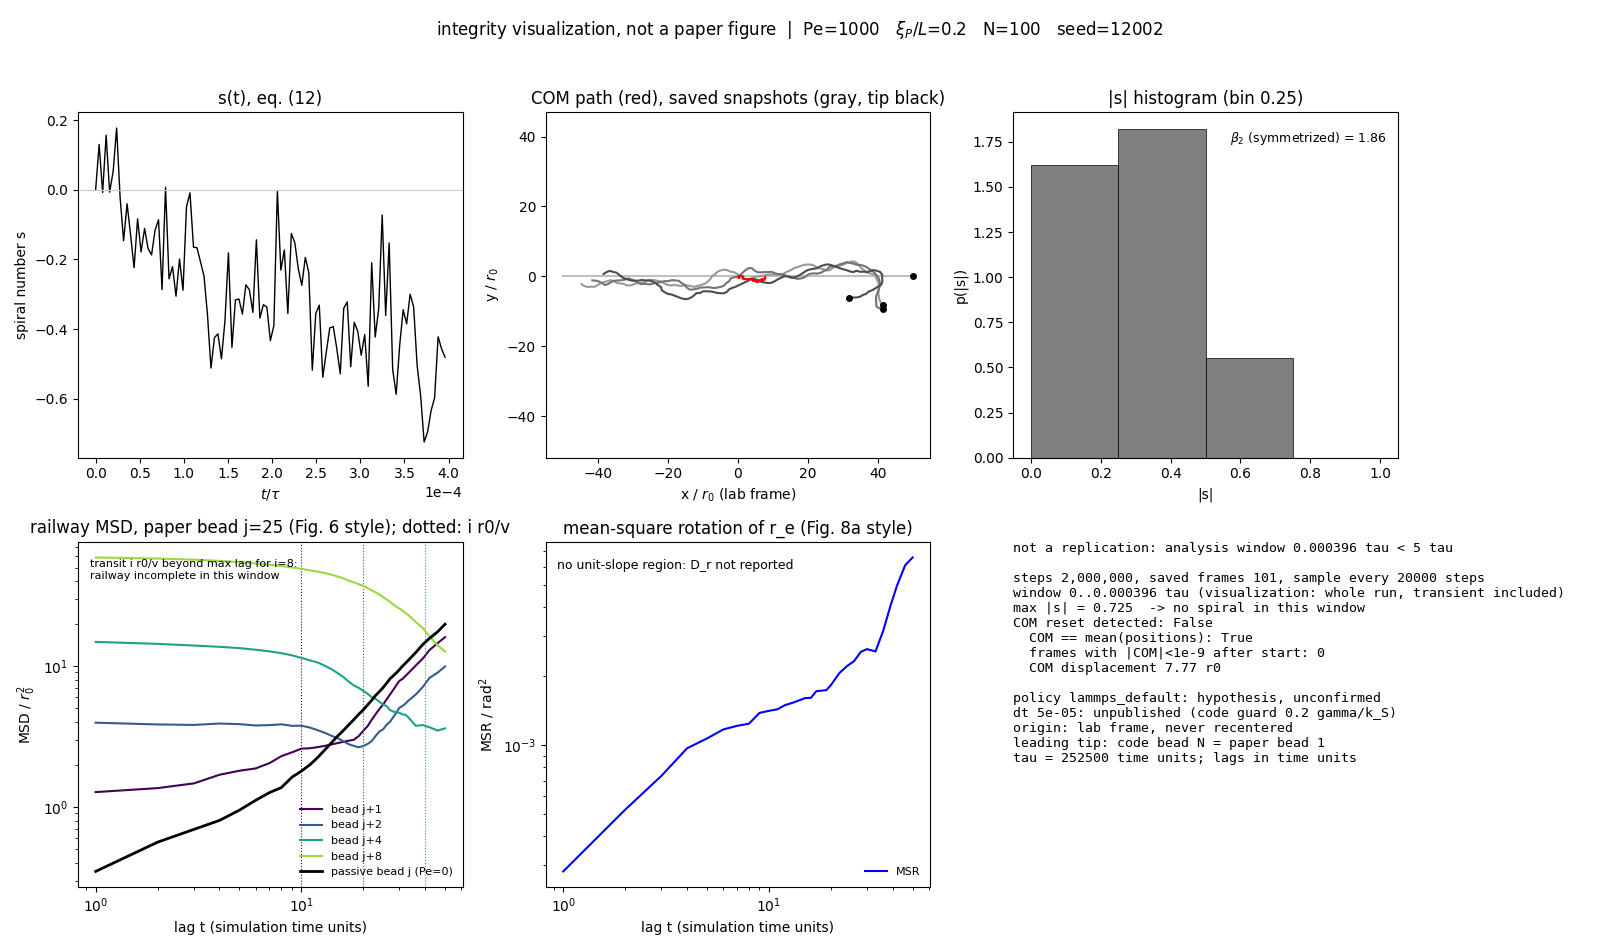
\includegraphics[width=\linewidth]{viz_weak.png}\\[0.5em]
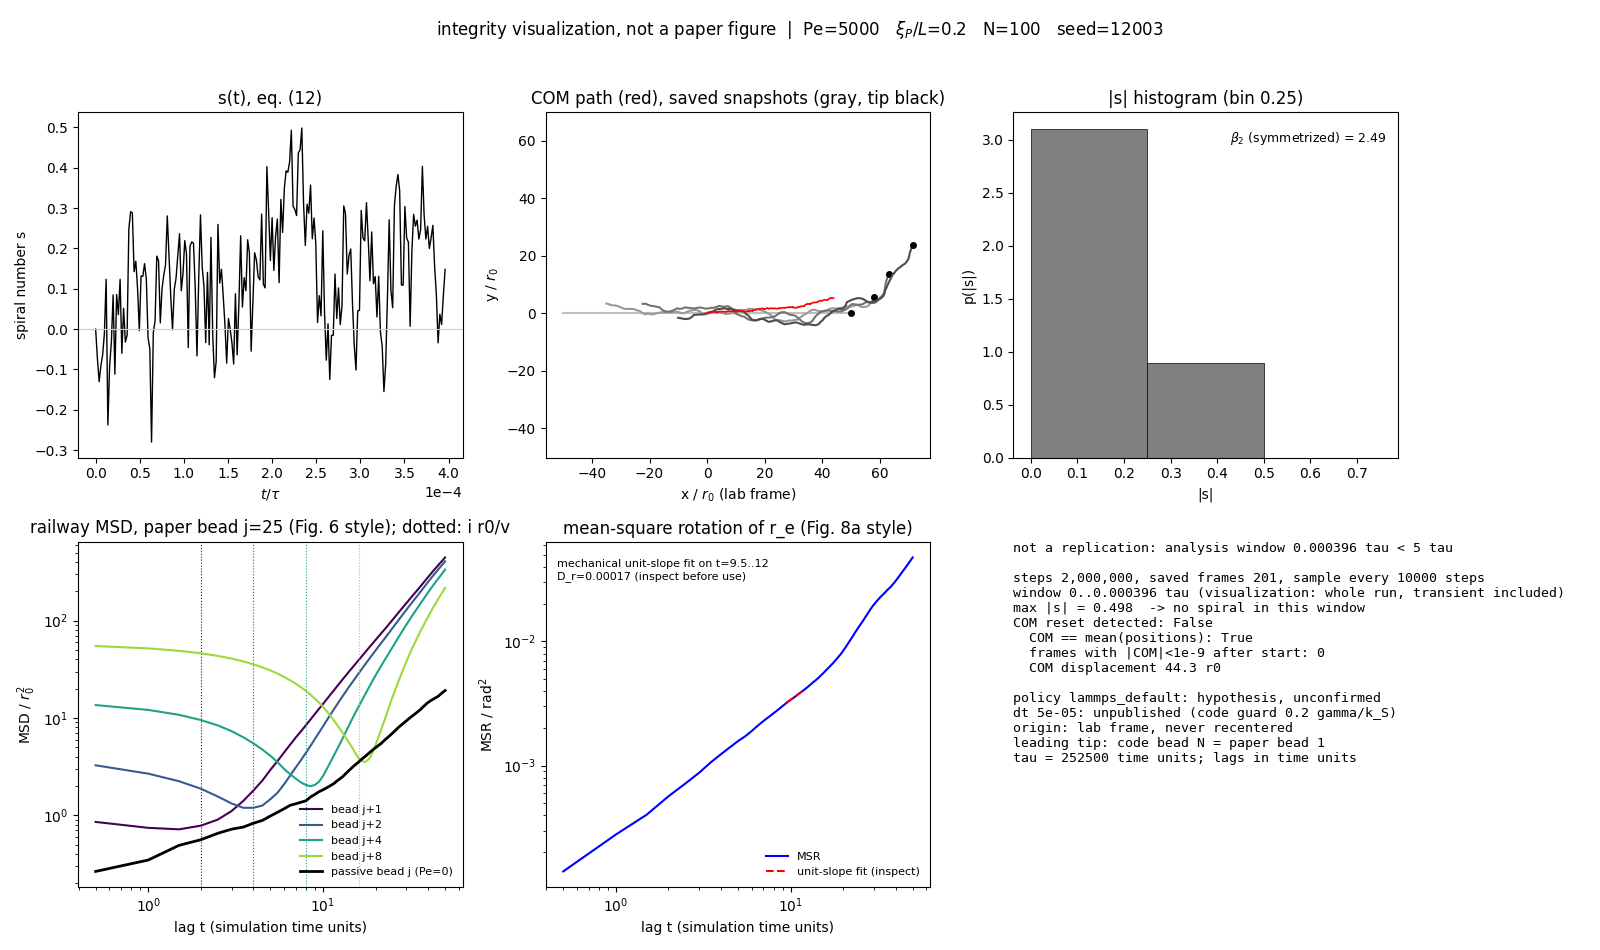
\includegraphics[width=\linewidth]{viz_strong.png}
\caption{Integrity panels (session 2): weak-spiral (top) and strong-spiral (bottom) presets over 100 time units. Panels: $\spn(t)$, COM path with snapshots,
$|\spn|$ histogram, railway MSD against the passive reference, MSR. Not paper figures.}
\end{figure}
\begin{center}\small
\begin{tabular}{lcccc}\toprule run & frames (film) & $\max|\spn|$ & COM displacement & COM reset? \\ \midrule
polymer $\Pe=200$ & 101 (101) & 0.427 & 2.58 & no \\ weak $\Pe=1000$ & 101 (101) & 0.725 & 7.77 & no \\
strong $\Pe=5000$ & 201 (101, stride 2) & 0.498 & 44.3 & no \\ \bottomrule\end{tabular}
\end{center}
No spiral formed in any of these windows; 100 time units is half a contour at $\Pe=5000$, so none was expected. The unit-slope rule again fitted early
crossovers: $9.6\times10^{-5}$ for the polymer run and $1.7\times10^{-4}$ for the strong run. Neither is a result.

\subsection{Session 3: the first formation gate}
Ten contours at $\Pe=5000$ ($4.04\times10^7$ steps, 401 frames at 0.025 contour, about 5--6 min each):
\code{lammps_default}/12003 had $\max|\spn|=1.68$ and failed; \code{paper_all_pairs}/12013 held $\spn\approx-4.1$ from 4.8 to 8.6 contours
(153 frames, 3.80 contours, $\max|\spn|=4.44$) and passed. Both COM checks were clean.
A $5\tau$ job was then launched with \code{paper_all_pairs} and the preset seed \emph{12003}, at the then-default cadence of $0.01\tau$.
This was the wrong job, as described next.

\subsection{Session 4: the wrong job, and the unconfounded gate}
\begin{warnbox}[title=Correction]
The job above used a seed (12003) that had been gated only under the other policy, where it failed. Its cadence ($0.01\tau=12.5$ contours) was also coarser than the only measured plateau (3.8 contours).
It was stopped at step $78\,780\,000$ (19.5 contours; last checkpoint $50\,500\,000$), was not resumed, and its folder is marked \code{STOPPED}.
\end{warnbox}
The gate was then repeated with the policy--seed pairs crossed:
\begin{figure}[H]\centering
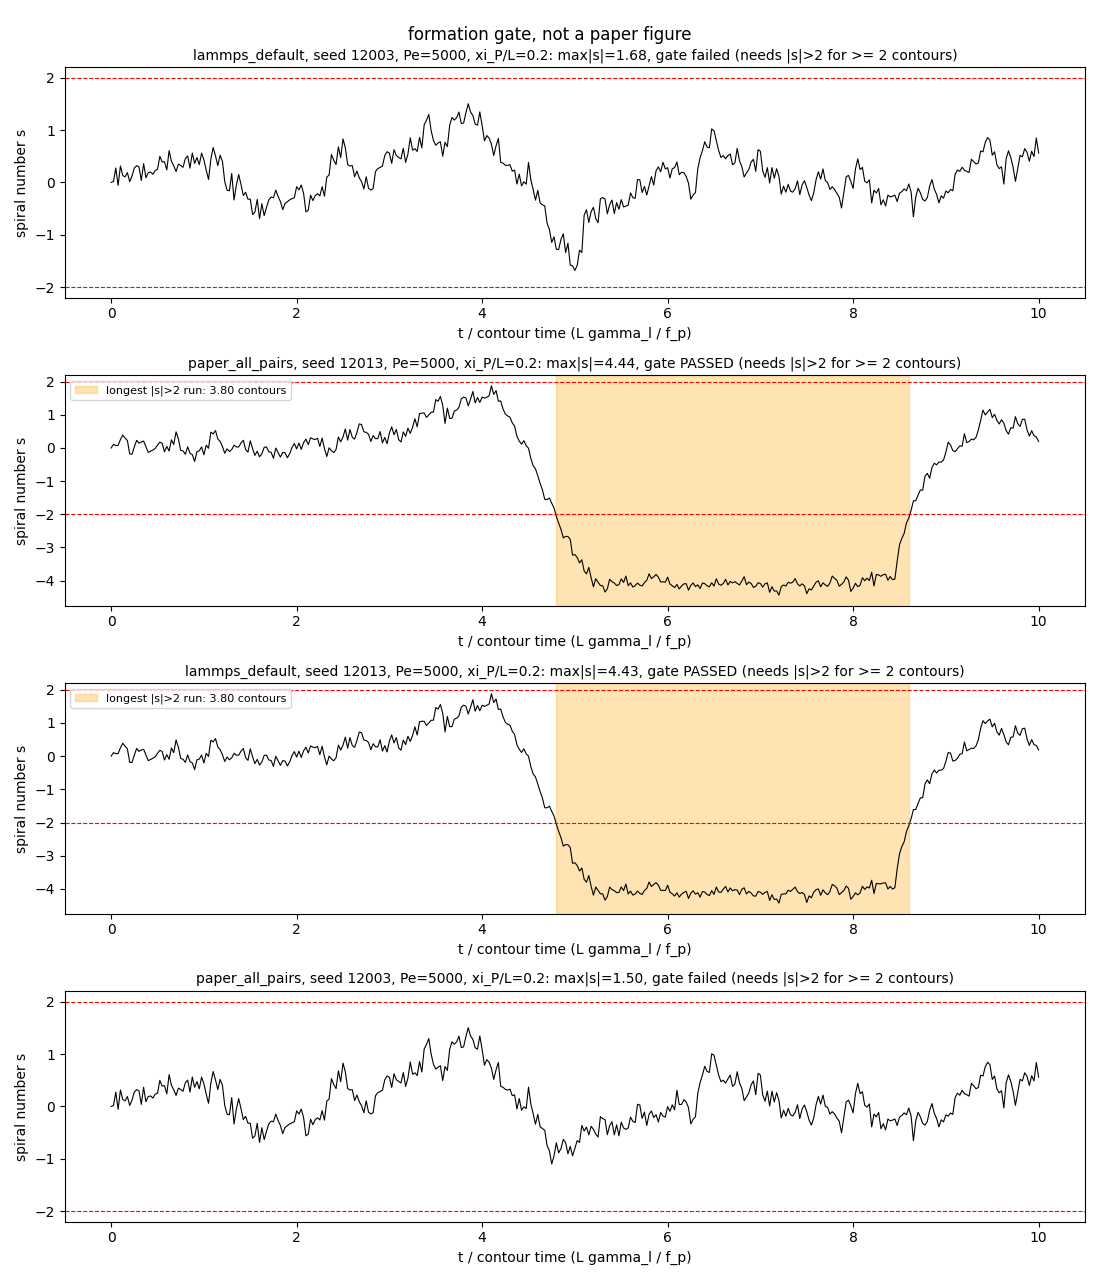
\includegraphics[width=0.84\linewidth]{gate4_s_t.png}
\caption{Unconfounded formation gate (10 contours each). Shaded: the longest $|\spn|>2$ run. Formation follows the seed, not the policy.}
\label{fig:gate4}
\end{figure}
\begin{center}\small
\begin{tabular}{llcccc}\toprule policy & seed & $\max|\spn|$ & longest $|\spn|>2$ run & COM check & gate\\ \midrule
\code{lammps_default} & 12003 & 1.68 & none & clean & fail\\
\code{paper_all_pairs} & 12013 & 4.44 & 3.80 contours (4.8--8.6) & clean & \textbf{pass}\\
\code{lammps_default} & 12013 & 4.43 & 3.80 contours (4.8--8.6) & clean & \textbf{pass}\\
\code{paper_all_pairs} & 12003 & 1.50 & none & clean & fail\\ \bottomrule\end{tabular}
\end{center}
\textbf{Interpretation.} Under a fixed seed, both policies consume the same noise stream; they differ only in the WCA forces between beads at most three bonds apart.
Formation is caused by tip--body contact at large separation, so the two trajectories stay close, and the gate cannot discriminate the policies.
Two seeds do not estimate a formation rate.

\begin{figure}[H]\centering
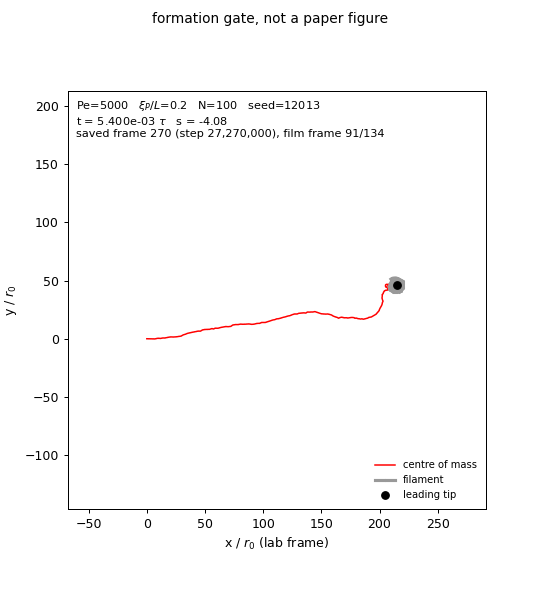
\includegraphics[width=0.42\linewidth]{frame_gate_lab.png}\hfill
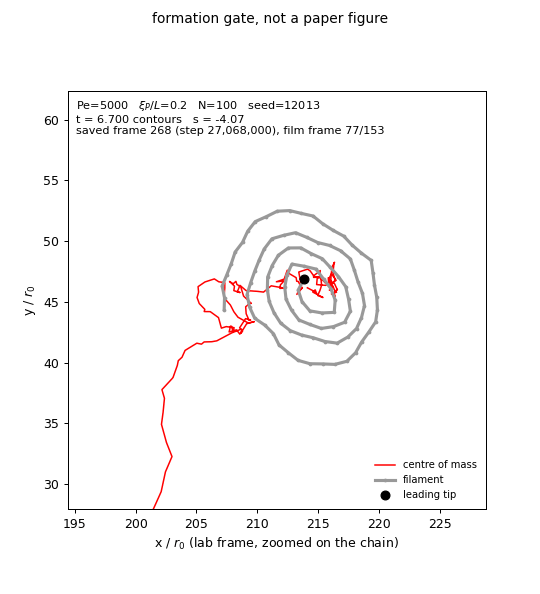
\includegraphics[width=0.42\linewidth]{frame_gate_plateau.png}
\caption{Seed 12013 gate film frames. Left: lab-frame box over the whole 250-$r_0$ trail ($\spn=-4.08$, $t=5.4\times10^{-3}\tau$). Right: zoom on the wound chain
(about four turns, leading tip black at the centre, COM wandering diffusively).}
\end{figure}

\subsection{Session 5--6: the $5\tau$ trajectory}
\begin{itemize}
\item \textbf{Configuration.} \code{strong_spiral}, \code{paper_all_pairs}, seed 12013; $25\,250\,000\,000$ steps; one frame every $1\,010\,000$ steps (0.25 contour), 25\,001 frames;
a checkpoint at every frame (about every 9\,s). Because the integrator is deterministic, the first 10 contours repeat the passing gate run exactly.
\item \textbf{Segment 1.} Started 2026-10-02 01:38:22 (+05:30). Stopped 03:38:09 at step $862\,540\,000$ ($0.171\tau$, 213.5 contours), with empty stderr and no reboot or sleep.
Fourteen seconds later the Windows log shows a service installation and the ``Claude'' service set to disabled.
The likely cause is an application update terminating its process tree; the timing is suggestive but not proof.
A read-only check showed the segment intact: 855 frames ending exactly at the checkpoint step, COM $\equiv$ mean of the positions, \code{complete=False}.
\item \textbf{Segment 2.} Resumed by the user (double-clicking \code{resume1.cmd}) on 2026-10-03 00:50:29 and completed 2026-10-05 06:03:49.
Segment wall time $191\,598$\,s (53.2\,h) for $2.4387\times10^{10}$ steps, i.e.\ $1.27\times10^5$ steps/s. The run reports a cumulative \code{wall_seconds} of $198\,785$\,s, because the checkpoint carries segment~1's time forward. The physics fingerprint is unchanged.
\item \textbf{Stitch.} 25\,001 frames from step 0 to $2.525\times10^{10}$, \code{complete=True}, bitwise-equal shared frame.
\end{itemize}

\begin{figure}[H]\centering
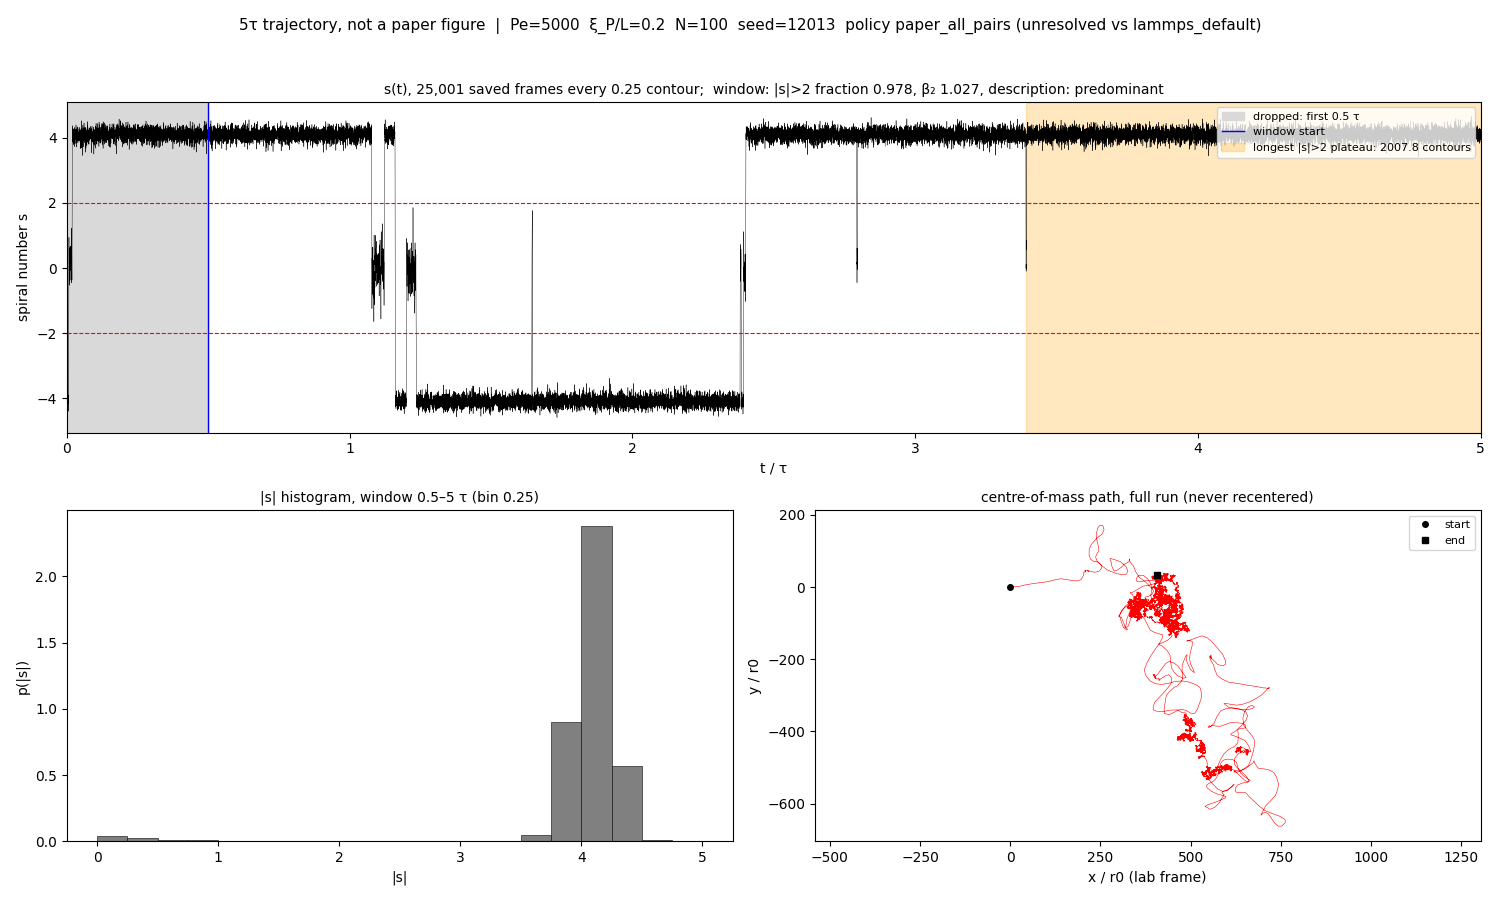
\includegraphics[width=\linewidth]{result_panel.png}
\caption{The $5\tau$ trajectory (seed 12013, $\Pe=5000$, $\xiP/L=0.2$). Top: $\spn(t)$, with the dropped first $0.5\tau$ shaded and the longest plateau highlighted.
Bottom left: window $|\spn|$ histogram. Bottom right: lab-frame COM path. Not a paper figure.}
\label{fig:result}
\end{figure}

\begin{table}[H]\centering
\caption{Verdict on the window $0.5$--$5.0\tau$ (22\,501 samples).}\label{tab:verdict}
\begin{tabular}{lr}\toprule
Description(s) & \textbf{predominant} \\
Fraction of samples with $|\spn|>2$ & 0.978 \\
Symmetrized $\beta_2$ & 1.027 \\
Longest plateau & $\geq$ 2007.75 contours ($\approx1.61\tau$; censored at run end) \\
COM MSD log--log slope & 1.001 \\
Unit-slope MSR region after $0.5\tau$ & none, so $D_r$ = null \\
$|\spn|$ in $[3.5,4.75)$ / $|\spn|<1$ & 97.7\% / 1.95\% (mode bin $[4.0,4.25)$) \\
Net COM displacement over $5\tau$ & 408.5 $r_0$ \\ \bottomrule
\end{tabular}
\end{table}

\begin{figure}[H]\centering
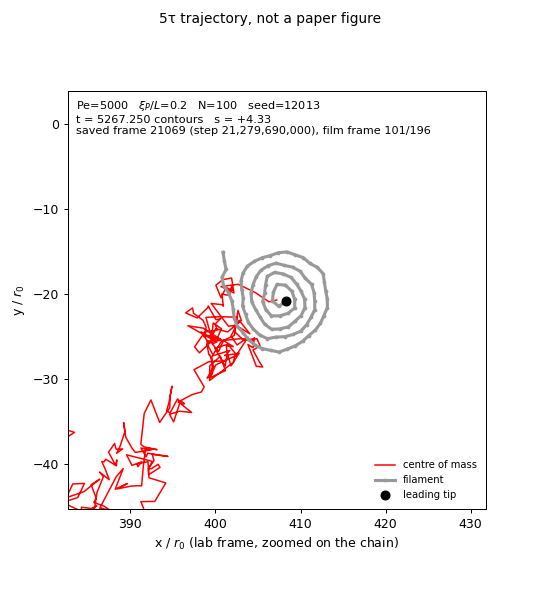
\includegraphics[width=0.45\linewidth]{frame_result_plateau.png}
\caption{Frame 101 of the 196-frame film of the longest plateau. The box follows the COM ($\pm24.6r_0$); the red trail starts at the plateau. $\spn=+4.33$ at $t=5267$ contours.}
\end{figure}

%=====================================================================
\section{Analysis and discussion}\label{sec:analysis}
%=====================================================================
\subsection{What the $5\tau$ trajectory shows}
\begin{itemize}
\item \textbf{Dynamics of $\spn$.}
\begin{itemize}
\item A spiral forms within the first few contours.
\item $\spn\approx+4$ holds until about $1.08\tau$; there are brief break-ups between $1.08$ and $1.24\tau$.
\item $\spn\approx-4$ holds from $1.24$ to about $2.4\tau$, then $\spn\approx+4$ to the end.
\item Single-frame dips occur near $2.8\tau$ and $3.39\tau$.
\item Spirals break up and re-form with either handedness. In the language of Fig.~4e this seed behaves like a light-red (break-up) strong-spiral point, not a dark-red (never breaks) one.
\end{itemize}
\item \textbf{Distribution.} The histogram has a minute low-$|\spn|$ peak (elongated state) and a dominant peak at $|\spn|\approx4$. Qualitatively this is the Fig.~4c description for $\Pe=5000$.
The low symmetrized $\beta_2$ ($\approx1$, the value for a two-point distribution at $\pm a$) is what the paper describes for spiral-dominated runs.
\item \textbf{Translation.} The COM path shows dense diffusive clusters while wound, linked by long directed excursions while elongated, the ``separated clusters'' of the Fig.~2 caption.
The long-lag COM MSD slope of 1.00 matches the paper's statement that translation in the spiral state is almost purely diffusive.
\item \textbf{Rotation.} No unit-slope MSR region appears. The paper likewise reports that the long-time MSR $\propto t$ regime ``could not be detected'' for runs with spontaneous break-up.
\end{itemize}

\subsection{Where this sits against the paper's claims}
\begin{center}\small
\begin{tabular}{p{0.42\linewidth}p{0.48\linewidth}}\toprule Paper's claim & Status here\\ \midrule
Tip collision winds the chain into a spiral at high $\Pe$, low $\xiP/L$ (Fig.~3a) & Observed (seed 12013), tip at the centre\\
Spiral state dominates at $\Pe=5000,\xiP/L=0.2$ (Fig.~2c, 4b--c) & Predominant on one seed over $4.5\tau$\\
$\beta_2\ll3$ when spirals dominate (Fig.~4d) & $\beta_2=1.03$ (one seed; values not compared numerically)\\
No spirals at $\Pe=200$ (Fig.~2a) & Consistent in a 100-time-unit run only\\
Railway motion; MSD minima touch passive (Fig.~6) & Seen qualitatively in a 100-time-unit run at $\Pe=1000,\xiP/L=0.2$\\
Formation depends on $(\Pe,\xiP/L)$ & Over 10 contours it depended on seed: 12003 did not wind\\
\bottomrule\end{tabular}
\end{center}

\subsection{Caveats that bound every statement}
\begin{enumerate}
\item \textbf{One seed, one point.} The verdict describes one trajectory. Seed-to-seed variability is unknown.
\item \textbf{Censoring.} The longest plateau ends with the run, so 2007.75 contours is a lower bound on its lifetime.
\item \textbf{Cadence.} At 0.25 contour per frame (50.5 time units), events shorter than a frame are invisible. Single-frame dips split plateaus under the consecutive-frame rule.
Fig.~6 needs about 2 time units per frame at $\Pe=5000$ and cannot be computed from this file.
\item \textbf{Policy unresolved.} The same seed gives the same formation under both policies; break-up statistics might differ, but that is untested.
\item \textbf{Timestep unpublished.} $\Delta t$ is a conservative guard. A different ESI value could shift break-up rates, which depend on tip curvature.
\item \textbf{Quantitative comparison absent.} The paper's figure values were not digitized, so ``consistent'' means qualitatively consistent.
\end{enumerate}

%=====================================================================
\section{Verification and audit status}\label{sec:tests}
%=====================================================================
\subsection{Test inventory (64 tests, all passing)}
Every new test has one assertion, and none merely checks that a number is finite.
\begin{longtable}{p{0.26\linewidth}p{0.06\linewidth}p{0.6\linewidth}}
\toprule file & n & what it establishes \\ \midrule\endhead
\code{test_forces.py} & 3 & finite-difference gradient of $U$; Newton's third law and net propulsion $f_p(\vect r_N-\vect r_0)$; policies differ\\
\code{test_engine_io.py} & 5 & chunk invariance (brute and Verlet); checkpoint round trip and fingerprint refusal; HDF5 sampling; overwrite refusal\\
\code{test_observables.py} & 6 & spiral number of an Archimedean spiral; Gaussian kurtosis; streaming moments; Kratky--Porod value; ballistic MSD slope; static $S(q,t)$\\
\code{test_paper.py}, \code{test_parameters.py} & 5 & Fig.~2 presets; $\tau=252\,500$; $5\tau$ step count; $\Delta t$ guard; $\kappa=20$, $f_p=0.5$, $\Flex=25\,000$\\
\code{test_origin.py} & 8 & COM not reset at the old boundary; stored positions equal an independent un-recentered integration; COM $\equiv$ mean of positions; recenter refused without offset; offset restores lab frame; resume equals uninterrupted (positions, angle); chunk size irrelevant\\
\code{test_figures.py} & 14 & unwrapping; railway minimum at transit; $D_r$ fit and its refusal; $\tau_S$ of an exponential; $S(q,t)$ translation phase; $\beta_2=1$ for constant $|\spn|$; histogram bins; leading-tip map; policy defaults agree; lags in time units; window; schema-2 refusal; plateau rule\\
\code{test_visualize.py} & 6 & refusal without \code{origin_convention}; frame cap; GIF frames are saved frames; reset detector; plateau films (fixed and following)\\
\code{test_reproduce_cli.py} & 10 & default 0.25 contour; $\tau$ and step units; resume equals uninterrupted; earlier segment kept; stitch equals uninterrupted; stitch refuses gap, overlap and a second origin; \code{--seed}\\
\code{test_verdict.py} & 7 & one synthetic series per description; $0.008\tau$ file refused; missing origin refused; altered COM refused; window starts at $0.5\tau$\\ \bottomrule
\end{longtable}

\subsection{Verified and unverified}
\begin{okbox}[title=Verified]
Force law against both sources; energy gradient; propulsion total; bitwise determinism under chunking, resume and stitching; lab-frame single origin across all stored frames and segments;
index map; every observable against an analytic or synthetic case; COM integrity of every production and gate file used.
\end{okbox}
\begin{warnbox}[title=Unverified or open]
\begin{itemize}
\item \textbf{Inputs.} ESI timestep; the original \code{special_bonds}; which policy the paper used.
\item \textbf{Generality.} Seed-to-seed reproducibility of formation and dominance.
\item \textbf{Comparison.} Quantitative agreement with any figure.
\item \textbf{Analysis.} Figs.~5, 8, 9, 10 analyses on the $5\tau$ file (the code exists; not yet run on it).
\end{itemize}
\end{warnbox}

\subsection{Known weaknesses in the tree}
\begin{itemize}
\item \code{paper.audit()} still reports \code{paper_faithful = (policy == 'lammps_default')}. It is a string comparison, not evidence; \code{paper.py} was outside the edit scope.
\item The $D_r$ unit-slope rule can lock onto a crossover; inspect the MSR before trusting a value.
\item GIF delays are quantised to 10\,ms, so the requested 12\,fps plays at 12.5\,fps (80\,ms per frame).
\item \code{analyze()} reads one file; multi-segment data must be stitched first.
\item An HDF5 file being written must not be opened by another process. HDF5 is not journaled, so a crash during a metadata write could corrupt a segment. The flush-before-checkpoint order limits the exposure.
\end{itemize}

\subsection{Incident log (errors made and how they were handled)}
\begin{enumerate}
\item \textbf{Test expectation error (session 1).} The first $S(q,t)$ translation test ignored the $|\rho_0(\hat q)|^2$ weighting. The test was corrected; the kernel was not changed.
\item \textbf{No-op typo (session 1).} \code{msr/2*2} in a fit call was removed before any run.
\item \textbf{Misleading diagnostic (session 1).} The smoke script first located the railway minimum with \code{argmin} of the MSD, which picks the short-lag $r_0^2$ plateau. It was replaced by the minimum of $\mathrm{MSD}_{j+i}/\mathrm{MSD}_\mathrm{passive}$.
\item \textbf{Wrong production job (session 3).} The job used seed 12003 at $0.01\tau$ cadence. It was stopped on request, not resumed, and superseded by session~4.
\item \textbf{Path slip (session 5).} A Unix-style path passed into Windows Python created \texttt{C:\textbackslash c\textbackslash\ldots}. It held only two scratch files, was verified, and was removed.
\item \textbf{Job killed by an application update (session 5--6).} The launch was a child of the app. The user restarted it from their own session; that is the recommended launch mode.
\item \textbf{Permissions.} The auto-mode classifier blocked registering a scheduled task, a detached launch from the agent, and the agent editing its own settings. These are by design.
\end{enumerate}

%=====================================================================
\section{Codebase reference}\label{sec:code}
%=====================================================================
\subsection{Layout}
\begin{longtable}{p{0.31\linewidth}p{0.06\linewidth}p{0.56\linewidth}}
\toprule module & lines & responsibility \\ \midrule\endhead
\code{parameters.py} & 64 & frozen \code{Parameters}: dimensionless inputs mapped to $\kappa,f_p,k_S,\gl,\tau,t_c$; \code{dt} guard; policy codes; SHA-256 \code{fingerprint()} of the canonical physics\\
\code{paper.py} & 10 & \code{FIG2} presets; \code{make(regime,policy)}; \code{audit()} (cost estimate)\\
\code{rng.py} & 22 & SplitMix64; 53-bit uniform; keyed Box--Muller \code{normal_pair(seed,step,bead)}\\
\code{forces.py} & 40 & all-pairs reference kernel with energies (used by tests)\\
\code{engine.py} & 95 & \code{straight()}; brute and Verlet integrators; opt-in recentering with offset; \code{benchmark()}\\
\code{simulator.py} & 51 & \code{run()}: sampling, angle unwrapping grid, flush, checkpoint, angle sidecar, resume\\
\code{io.py} & 51 & \code{strict_json}; \code{H5Trajectory} (schema 3, provenance attributes)\\
\code{checkpoint.py} & 18 & atomic \code{npz} save; load with schema and fingerprint checks\\
\code{observables.py} & 85 & every observable in Section~\ref{sec:observables}\\
\code{moments.py} & 10 & streaming fourth moment (symmetrized)\\
\code{analysis.py} & 87 & \code{analyze()}: the second program, a window-explicit Figs.~4--10 input set\\
\code{stitch.py} & 61 & \code{read_segments}, \code{write_stitched}\\
\code{visualize.py} & 141 & films, panels, \code{plateau_film}, COM reset check\\
\code{cli.py} & 61 & command-line interface (Section~\ref{sec:ops})\\
\code{hardware.py}, \code{taichi_backend.py} & 22 & probes only; Vulkan is never used in production\\ \midrule
\code{tests/smoke_integrity.py} & 36 & smoke driver: active run, passive run, analysis\\
\code{tests/formation_gate.py} & 39 & gate evaluator and multi-curve $\spn(t)$ plot\\
\code{tests/verdict.py} & 75 & verdict program\\
\code{tests/result_figures.py} & 41 & $5\tau$ result panel and plateau film\\ \bottomrule
\end{longtable}

\subsection{Data formats}\label{sec:formats}
\textbf{Trajectory (HDF5, schema 3).}
\begin{itemize}
\item Datasets (gzip-compressed, extendable): \code{step} (int64), \code{time}, \code{time_tau}, \code{spiral}, \code{com}$[n,2]$, \code{end_to_end}$[n,2]$, \code{ee_angle} (unwrapped), \code{rg}, \code{positions}$[n,N+1,2]$.
\item Attributes: \code{complete}, \code{schema}, \code{fingerprint}, \code{parameters_json}, \code{origin_convention}, \code{leading_tip}, \code{nonbonded_policy}, \code{nonbonded_policy_status}, \code{timestep_status}, \code{start_step}, \code{sample_every}, \code{ee_angle_branch}, \code{ee_angle_unwrap_every_steps}, \code{ee_angle_max_increment_rad}.
\item A stitched file adds \code{stitched_from}.
\end{itemize}
\textbf{Checkpoint (\code{.npz}).} \code{x}, \code{step}, \code{wall_seconds}, \code{schema}, \code{fingerprint}. Loading refuses a fingerprint mismatch.
\textbf{Angle sidecar (\code{.angle.json}).} \code{step}, \code{fingerprint}, \code{ee_angle}.
\textbf{Verdict (\code{.json}).} \code{duration_tau}, \code{window}, \code{fraction_abs_s_gt_2}, \code{longest_plateau_contours}, \code{beta2_symmetrized}, \code{abs_s_histogram}, \code{com_msd_loglog_slope}, \code{msr_unit_slope_region_exists}, \code{D_r}, \code{descriptions}, \code{description_rules}, plus provenance fields.

%=====================================================================
\section{Operator's guide}\label{sec:ops}
%=====================================================================
\subsection{Installation}
From the tree root (\code{spin-chain-paper-v2/spin-chain-paper-v2}):
\begin{lstlisting}[style=sh]
uv venv -p 3.11 .venv311
uv pip install -p .venv311/Scripts/python.exe -r requirements.txt
set PYTHONPATH=src            (cmd.exe)   |   export PYTHONPATH=src   (bash)
.venv311\Scripts\python.exe -m pytest -q   # expect 64 passed
\end{lstlisting}

\subsection{Command reference (\code{python -m spinchain <cmd>})}
\begin{longtable}{p{0.2\linewidth}p{0.74\linewidth}}\toprule command & purpose and key flags\\ \midrule\endhead
\code{benchmark} & throughput of brute and Verlet kernels: \code{--steps}, \code{--regime}, \code{--policy}\\
\code{paper-audit} & benchmark plus a cost estimate for $\tau$ units and replicates\\
\code{headless} & a single trajectory of fixed length: \code{--regime --steps --sample-every --output [--checkpoint --resume --overwrite --policy --wall-limit --no-positions]}\\
\code{paper-reproduce} & paper-length runs: \code{--regime --tau --replicates --seed --policy --sample-every (e.g. 0.25contour) --output-dir --i-know [--resume --overwrite]}\\
\code{analyze} & \code{analyze()} on one file: \code{--structure --json-out --window-start-tau --window-end-tau --window-reason}\\
\code{visualize} & film and panel: \code{--passive --out-dir --fps --max-frames}\\
\code{hardware}, \code{vulkan-probe} & environment probes\\ \bottomrule
\end{longtable}
Scripts in \code{tests/} (run directly):
\begin{itemize}
\item \code{smoke_integrity.py --regime R --steps S --sample-every K};
\item \code{formation_gate.py [--name N] [--no-films] RUN.h5 ...};
\item \code{verdict.py STITCHED.h5 --out V.json};
\item \code{result_figures.py STITCHED.h5 V.json}.
\end{itemize}

\subsection{The production workflow}
\begin{enumerate}
\item \textbf{Benchmark} the point and policy, then budget: steps $=\lceil 5\tau/\Delta t\rceil$ divided by steps/s.
\item \textbf{Gate} (optional but recommended): a 10-contour \code{headless} run per policy and seed with about 400 frames, then \code{formation_gate.py}.
\item \textbf{Launch from your own terminal}, not from the agent (an app update can kill the agent's child processes). For example:
\begin{lstlisting}[style=sh]
python -m spinchain paper-reproduce --regime strong_spiral --policy paper_all_pairs --seed 12013 --tau 5 --replicates 1 --output-dir output/reproduction/paper_all_pairs-seed12013 --i-know
\end{lstlisting}
\item \textbf{Monitor.} Read only the log (\code{progress: step=... contours=... tau=...}) and the angle sidecar. Never open the running \code{.h5}.
\item \textbf{Recover.} If the process dies, rerun the same command with \code{--resume}. It continues from the last checkpoint (losing at most one frame interval) into a new \code{.from<step>.h5} segment. \code{resume1.cmd} wraps this with log redirection for double-click use.
\item \textbf{Completion} is a log ending in \code{"completed": true}. Then stitch, verdict and figures:
\begin{lstlisting}[style=sh]
python -c "import glob;from spinchain.stitch import write_stitched;print(write_stitched(glob.glob('output/reproduction/paper_all_pairs-seed12013/strong_spiral-seed12013*.h5'),'output/reproduction/strong_spiral-paper_all_pairs-seed12013-stitched.h5'))"
python tests/verdict.py output/reproduction/strong_spiral-paper_all_pairs-seed12013-stitched.h5 --out output/reproduction/verdict-paper_all_pairs-seed12013.json
python tests/result_figures.py output/reproduction/strong_spiral-paper_all_pairs-seed12013-stitched.h5 output/reproduction/verdict-paper_all_pairs-seed12013.json
\end{lstlisting}
\end{enumerate}

\subsection{Troubleshooting}
\begin{description}[style=nextline]
\item[\code{FileExistsError}] Output exists. Use a new path, or \code{--overwrite} only if you intend to discard it. Never combine \code{--overwrite} with resuming data you want to keep.
\item[\code{checkpoint physics fingerprint mismatch}] Different parameters, policy or seed from the run that wrote the checkpoint.
\item[Stitch refuses gap, overlap or origin] Segments are missing, duplicated, or come from different runs; do not force them.
\item[Verdict refuses] Too short, an altered COM, an unlabelled frame, or non-uniform cadence; the message names the cause.
\item[Slow runs] Use mains power and the ``Best performance'' power mode. Spiral states are about $10$--$20\%$ slower (more pair contacts). Run independent jobs on separate cores.
\item[Windows paths] In Python on Windows use \code{C:/...} or raw strings; \code{/c/...} is interpreted as \texttt{C:\textbackslash c\textbackslash\ldots}.
\end{description}

%=====================================================================
\section{Next directions}\label{sec:next}
%=====================================================================
\begin{enumerate}
\item \textbf{Unblock inputs (hours).}
\begin{itemize}
\item Obtain the article ESI (``details of the simulations''); it may contain the timestep table or the LAMMPS input.
\item Digitize Figs.~4d, 5, 8b and 10b to obtain numeric targets.
\item Profile the kernel for bitwise-identical speedups.
\end{itemize}
\item \textbf{Regime contrast and robustness (one parallel batch, about 3 days).} All runs at $5\tau$, 0.25-contour cadence, $\xiP/L=0.2$:
\begin{itemize}
\item $\Pe=200$ (seed 12001);
\item $\Pe=1000$ (seed 12002);
\item $\Pe=5000$ seed 12003;
\item $\Pe=5000$ with a new seed;
\item $\Pe=5000$ seed 12013 under \code{lammps_default}: a policy comparison on break-up and lifetime statistics, not on formation.
\end{itemize}
\item \textbf{Dynamics figures.}
\begin{itemize}
\item Fig.~6: $\xiP/L=0.3$, $\Pe=1000$, dense short runs.
\item Figs.~8--9: Pe sweeps.
\item Fig.~10: $\xiP/L=1$.
\end{itemize}
\item \textbf{Phase diagram.} About 40--60 grid points $\times$ about 2.5 days each, i.e.\ 100--150 core-days. Choose one row ($\xiP/L=0.2$ across Pe) or move to a cluster.
\end{enumerate}

\appendix
\section{Key numbers}
\begin{center}\small
\begin{tabular}{ll}\toprule
$\tau$ & 252\,500 time units $=5.05\times10^9$ steps\\
$5\tau$ & $2.525\times10^{10}$ steps\\
contour time at $\Pe=5000$ & 202 time units $=4.04\times10^6$ steps\\
production cadence & $1\,010\,000$ steps $=0.25$ contour $=2\times10^{-4}\tau$\\
Verlet throughput & $1.0$--$1.4\times10^5$ steps/s per core\\
$5\tau$ wall time (observed) & $\approx55.2$\,h of compute ($7\,187$\,s $+$ $191\,598$\,s; cumulative \code{wall_seconds} $=198\,785$)\\
stitched file & 25\,001 frames, $\approx33$\,MB (gzip)\\ \bottomrule
\end{tabular}
\end{center}

\section{Notes written during the work}
The tree root holds the session notes this report consolidates:
\begin{itemize}
\item \code{REPRO_NOTE.md}: origin fix and observables;
\item \code{VIZ_NOTE.md}: visualizer;
\item \code{PRODUCTION_NOTE.md}: first gate, now superseded;
\item \code{CADENCE_NOTE.md}: unconfounded gate, cadence, stitch;
\item \code{VERDICT_PLAN.md}: verdict design, interruption and resume;
\item \code{RESULT_NOTE.md}: the $5\tau$ result.
\end{itemize}

\vspace{1em}
\begin{keybox}
\textbf{Bottom line.} The integrator, file format and analysis chain are now trustworthy and tested. One $5\tau$ trajectory at the strong-spiral point is spiral-predominant on its seed. That is evidence consistent with Fig.~2c, and \NR.
\end{keybox}

\end{document}
